\documentclass[a4paper,12pt,oneside]{article}

% Imported packages
\usepackage[english]{babel}
\usepackage[T1]{fontenc}
\usepackage[utf8]{inputenc}
\usepackage{amssymb}
\usepackage{amsmath}
\usepackage{bm}
\usepackage{listings}
\usepackage{graphicx}
\usepackage{geometry}
\usepackage{float}
\usepackage{subfigure}
\usepackage{wrapfig}
\usepackage{color}
\usepackage{comment}
\usepackage{hyperref}

% Margin dimensions settings
\geometry{a4paper,top=2cm,bottom=2cm,left=2cm,right=2cm,%
	heightrounded,bindingoffset=5mm}

% x bar for UTF-8 encoding
\DeclareUnicodeCharacter{304}{$ \bar{x} $}

% Enumeration settings
\renewcommand\thesubsection{\thesection.\alph{subsection}}

% Code visualization settings
\lstset{basicstyle=\small\ttfamily}

% Code design settings
\lstset{language=Matlab}

% Included images path
\graphicspath{{Images/}}

% Document information
\title{Fundamentals of Vibration Analysis and Vibroacoustics \\
	Module 2 - Vibroacoustics of Musical Instruments \\
	Assignment 1 - Experimental modal analysis of a violin}
\author{Bombaci Nicola 10677942 \\
	Fantin Jacopo 10591775 \\
	Intagliata Emanuele 10544878}
\date{June 2020}


\begin{document}

\maketitle

\vspace{100pt}

\section{Matlab code for mode identification}

Like we did for the modal parameter identification assignment, we first need an initial guess to start from.

\subsection{Initial guess for minimization process}



\begin{figure}[h]
	\hspace{-70pt}
	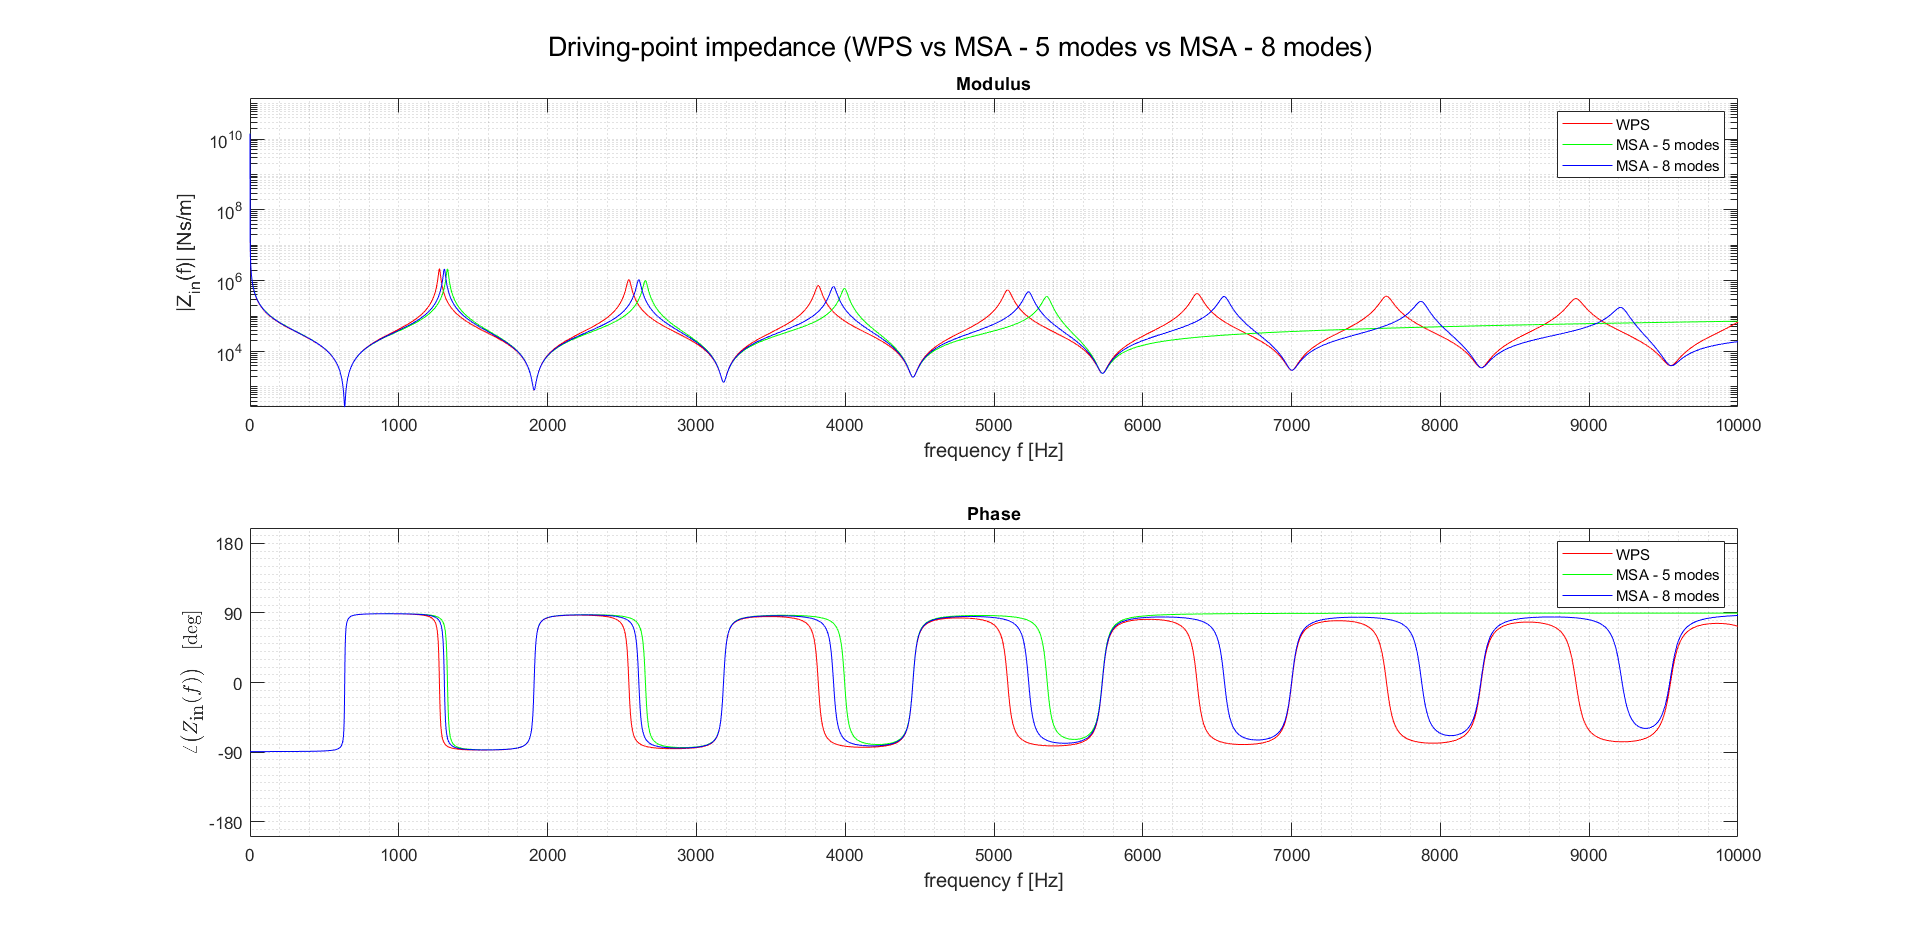
\includegraphics[scale=0.4]{impedance_wps_vs_msa}
\end{figure}


\end{document}